\chapter{Coupled Results}
\label{ch:coupledResults}

\section{Power Reactor Modeling}
\label{sec:power_reactor_modeling}
  The motivation for this work is to model nuclear power reactors with
  multiphysics feedback. This has been accomplished by modeling power
  distribution with the multigroup neutron diffusion equation solved via the
  Finite Element Method (FEM) (\chref{ch:neutronDiffusion}), axial heat
  convection and radial heat conduction models (\chref{ch:thermalHydraulics}),
  and simplified thermal expansion modeling (\chref{ch:thermalExpansion}).
  Combined, these effects will provide feedback which can be estimated in the
  model. 
  
  A realistic reactor benchmark is provided and modeled \sref{sec:abr}.
  Reactivity coefficients describing system responses are defined in
  \sref{sec:reactivity_coefficients}. Results are presented in
  \sref{sec:results}.

\section{Advance Burner Reactor -- MET 1000}
\label{sec:abr}
  This problem is proposed by Organisation for Economic Co-operation and
  Development Nuclear Energy Agency (OECD NEA) in \cite{abr}. The Advanced
  Burner Reactor (ABR) is fueled with a ternary metallic fuel and has a 1000
  \units{MWth} rating. This is a medium-sized metalic reactor with a total of
  180 assemblies and is 4.8 \units{m} tall. The benchmark is fully specified and
  thirty-one independent results are submitted. Each submission has generated
  its own cross-sections. Submissions include a solution using \dif.

  The materials in the benchmark are shown in \fref{fig:abr_materials}. Fast
  neutron flux is shown to peak in the core center and thermal neutron flux is
  shown to peak in the structural material surrounding the core in
  \fref{fig:abr_fluxes}.

  \begin{figure}
    \centering
    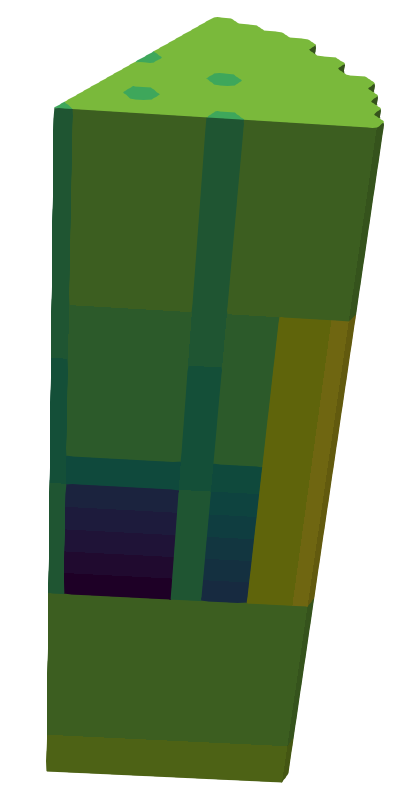
\includegraphics[width=0.4\textwidth]{abr_materials}
    \caption{Materials in ABR.}
    \label{fig:abr_materials}
  \end{figure}

  \begin{figure}
    \centering
    \subfloat[$\phi_{1}$]{
      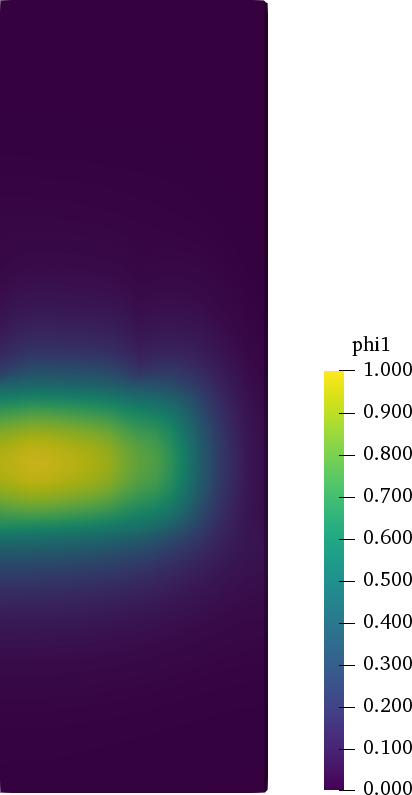
\includegraphics[width=0.25\textwidth]{abr_phi_nod_group1}}
    \hspace{0.2in}
    \subfloat[$\phi_{33}$]{
      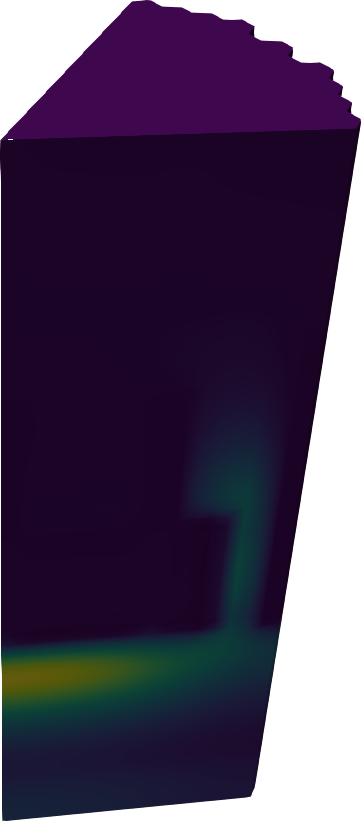
\includegraphics[width=0.25\textwidth]{abr_phi_nod_group33}}
    \caption{Multigroup Neutron Flux in ABR.}
    \label{fig:abr_fluxes}
  \end{figure}

\section{Reactivity Coefficients}
\label{sec:reactivity_coefficients}
  % give formulae for everything

\section{Results}
\label{sec:results}

